% !TEX root = ../SystemTemplate.tex

\chapter{Overview and concept of operations}

\section{Scope}
This section covers an overview of the Crowd Science Mapper. This section will contain information about the prupose, goals, major system components, and technology used.

\section{Purpose and System Goals}
The purpose of of this system is to provide a generic crowdsourcing website, where ordinary citizens can report events such as butterfly or bird sightings; where researchers can view event reports; and administrators can edit event report data sets and make changes to event data.  The goal of this system is to fulfill this purpose.

\subsection{Event Reporting}
Ordinary citizens will be able to log in and report events that can then be viewed by researchers, academics and other ordinary citizens. 

\subsection{Event Set Editing}
Administrators can edit existing events sets to refine what users report, and create new event sets to allow users to start reporting events.  Administrators will be able to moderate the events that users report.

\subsection{Event Viewing}
Researchers will be able to view events in a map representation, with greater event detail provided below the map. This project may be extended to include database queries about the event sets.

\section{System Overview and Diagram}
The webpage will consist of the major components. The main page will contain a map and detailed list of events for the selected event set. There will be a button on the main page that will take the user to a reporting interface. The user can login, and if the user is an administrator, the main page will contain buttons leading to the pages for editing and creating event sets and editing individual events. See Figure~\ref{mainpage}..

\begin{figure}[tbh]
\begin{center}
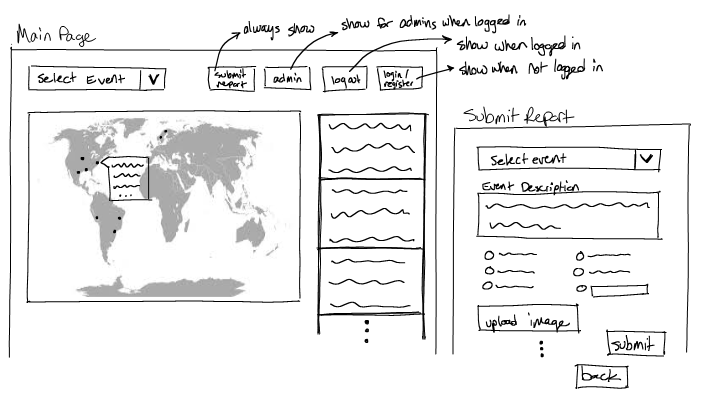
\includegraphics[width=0.75\textwidth]{./Images/crowdscience_mainpagesketch.png}
\end{center}
\caption{Design of Crowd Science Main Page\label{mainpage}}
\end{figure}

\section{Technologies Overview}
This section contains a list of specific technologies used to develop the system.  See Table~\ref{technologies}.  

\begin{table}[tbh]
\caption{Technologies Used \label{technologies}}
\begin{center}
\begin{tabular}{|>{\raggedright}p{2cm}|>{\raggedright}p{4cm}|>{\raggedright}p{4cm}|>{\raggedright}p{4cm}|}

  \hline
\textit{\textbf{Technology}} &  \textit{\textbf{Description}} & \textit{\textbf{Reference Material}} & \textit{\textbf{System Usage}}\tabularnewline
\hline
 \textit{\textbf{Apache 2.0}} & \textit{Used for website server hosting.} & \textit{\url{http://httpd.apache.org/docs/2.0/}} & \textit{Used to host Crowd Science Mapper website.}\tabularnewline
\hline
 \textit{\textbf{HTML}} & \textit{Hypertext Markup Language, basic webpage scripting language.} & \textit{\url{http://html.net/}} & \textit{Used to tie together JavaScript, PHP, and CSS webpages.}\tabularnewline
 \hline
  \textit{\textbf{JavaScript}} & \textit{More advanced language to create more complex objects.} & \textit{\url{http://html.net/}} & \textit{Used to create more complex objects, such as the event map.}\tabularnewline
 \hline
  \textit{\textbf{PHP}} & \textit{Hypertext Preprocesser, used with HTML to provide stateful webpages.} & \textit{\url{http://html.net/}} & \textit{Used to send and recieve information from the Mongo Database.}\tabularnewline
 \hline
  \textit{\textbf{CSS}} & \textit{Cascading Style Sheet, used to create a unified look and feel for websites.} & \textit{\url{http://html.net/}} & \textit{Used to create look and feel of Crowd Science Mapper.}\tabularnewline
 \hline
  \textit{\textbf{Mongo Database}} & \textit{Used to store information.} & \textit{\url{http://www.mongodb.org/}} & \textit{Used to store user login information and event reports.}\tabularnewline
\hline
\end{tabular}
\end{center}
\end{table}

